%%--------------------------------------------------------------------------
%% INTERFACCIA UTENTE
%%--------------------------------------------------------------------------



\subsection{User Interface}
\label{chap:ui}

Come anticipato nel capitolo \ref{chap:game_logic}, l'interfaccia grafica del gioco è gestita quasi interamente da \code{Fragments}, che rispondono agli eventi pubblicati sul Bus dall'activity \code{PlayActivity} aggiornando i loro componenti.\\
I due principali \code{Fragments} sono \code{WordsFragment} e \code{SyllablesFragment} (vedi figura \ref{fig:fragments}), che si occupano rispettivamente di gestire la porzione di schermo contenente le parole, e la porzione contenente le sillabe disponibili.

\begin{figure}[h!]
\label{fig:fragments}
  \centering
    \centering{
      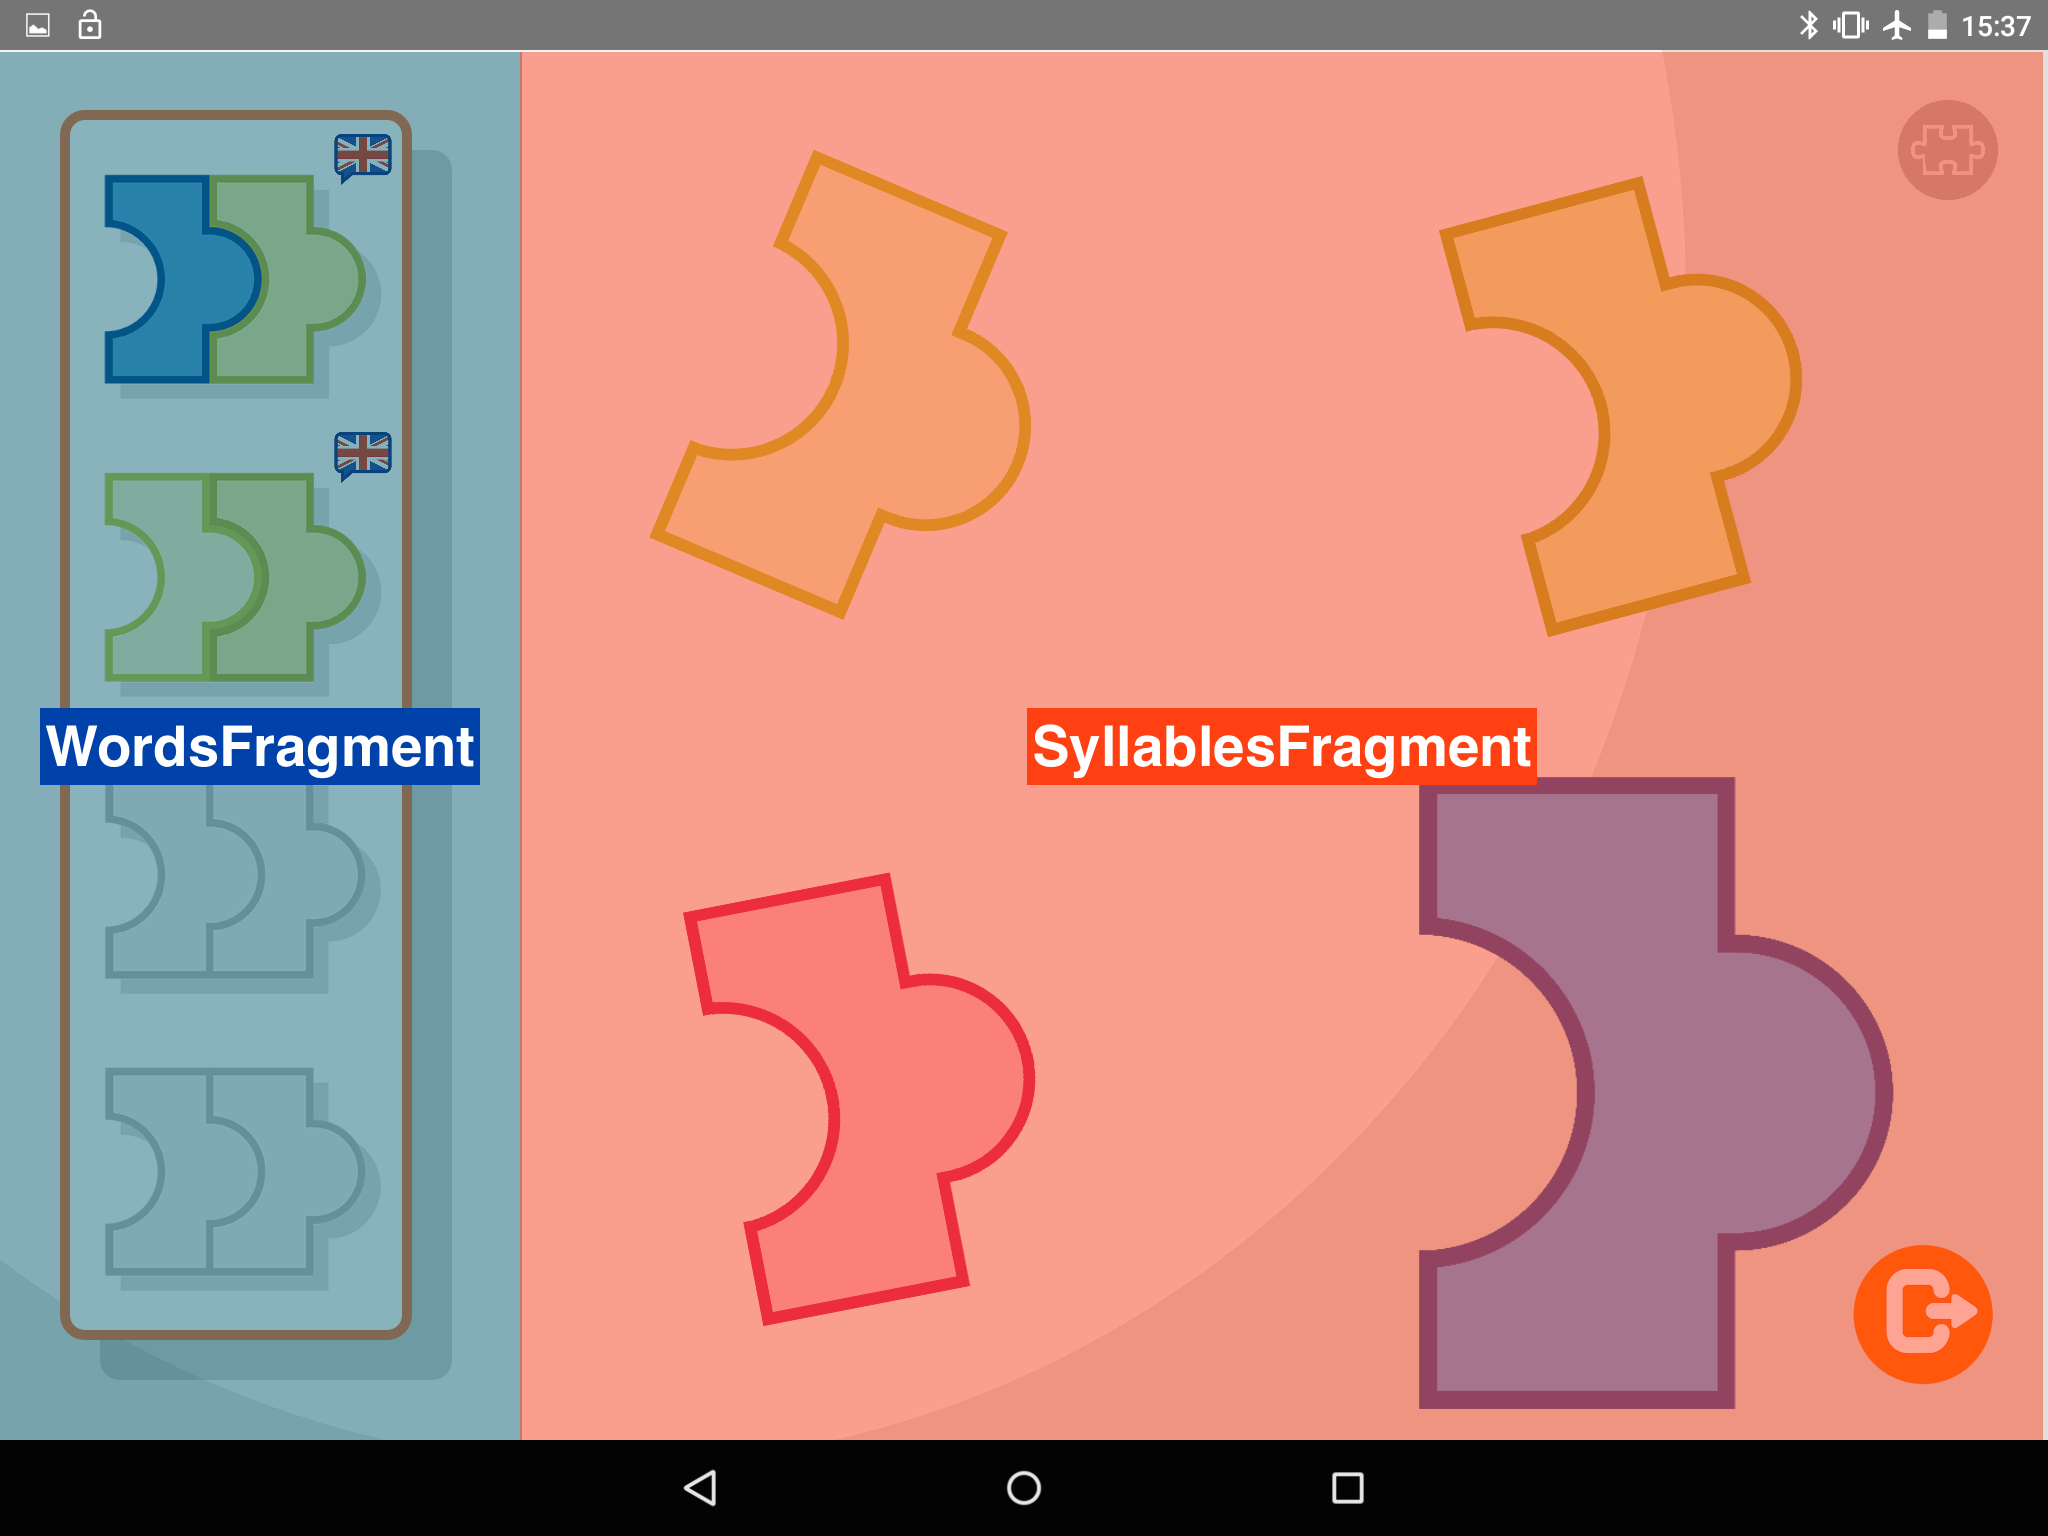
\includegraphics[width=\textwidth]{fragments.png}}
  \caption{Fragments della schermata di gioco}
\end{figure}


\subsubsection{WordsFragment}
\label{sec:words_fragment}
\code{WordsFragment} si occupa di gestire la parte di interfaccia grafica che rigurda le parole già trovate e quella ancora da trovare.\\
Esso presenta una lista verticale di ``slot'' che possono essere ``vuoti'', o ``riempiti'' con le tessere di puzzle corrispondenti alle sillabe che formano la parola. Viene inoltre mostrata accanto ad ogni slot ``pieno'' una bandiera inglese che se toccata permette di ascolare il suono della parola tradotta in inglese.\\
Il metodo \code{initUI()} si occupa, dato il numero di parole da trovare e la dimensione dello schermo (calcolata a runtime), di calcolare la dimensione degli slot corretta per gli slot con lo scompo di riempire al meglio lo spazio disponibile.\\
Le immagini degli slot sono fornite come file PNG all'interno della cartella \code{assets} e vengono caricate dinamicamente come Bitmap della dimensione corretta (per risparimare memoria) dal metodo \code{loadWordBitmap()}.\\
Il \code{Fragment} è sottoscritto all'evento \code{StateUpdatedEvent} in modo da reagire ai cambiamenti di stato della partita, come il ritrovamento di una nuova parola.

\subsubsection{SyllablesFragment}
\label{sec:syllables_fragment}

\code{SyllablesFragment} si occupa di gestire la parte di interfaccia grafica che rigurda le sillabe disponibili nella pagina corrente.\\
Esso presenta una griglia sparsa di 2 o 4 tessere di puzzle colorate rappresentanti ognuna una sillaba. Se toccate le tessere vengono selezionate e si ``alzano'' per restituire un feedback della selezione e riproducono il suono della sillaba a cui sono associate.\\
Al pari di \code{WordsFragment} calcola la dimensione corretta delle immagini e le carica come Bitmap.
